%%%
%% v1.8 [2011/12/16]
\documentclass[letter]{ieice}%不是paper
%\documentclass[tutorial]{ieice}
%\documentclass[invited]{ieice}
%\documentclass[survey]{ieice}
%\documentclass[invitedsurvey]{ieice}
%\documentclass[review]{ieice}
%\documentclass[letter]{ieice}
%\documentclass[brief]{ieice}
%\usepackage{cTex}
\usepackage{amssymb}
\usepackage{amsmath}
%\usepackage{enumerate}
%\usepackage{geometry}
\usepackage{graphicx}%
\usepackage{latexsym}%
%\usepackage[fleqn]{amsmath}
\usepackage[varg]{txfonts}%

\setcounter{page}{1687}%页码

%% <local definitions>
\def\ClassFile{\texttt{ieice.cls}}
\newcommand{\PS}{{\scshape Post\-Script}}
\newcommand{\AmSLaTeX}{%
 $\mathcal A$\lower.4ex\hbox{$\!\mathcal M\!$}$\mathcal S$-\LaTeX}
\def\BibTeX{{\rmfamily B\kern-.05em
 \textsc{i\kern-.025em b}\kern-.08em
  T\kern-.1667em\lower.7ex\hbox{E}\kern-.125emX}}
\hyphenation{man-u-script}
\makeatletter
\def\tmpcite#1{\@ifundefined{b@#1}{\textbf{?}}{\csname b@#1\endcsname}}%
\makeatother
%% </local definitions>

\field{D}
\vol{95}
\no{6}
%\SpecialSection{Letter}
%\SpecialIssue{}
\title[How to Use the Class File (\ClassFile)]
      {Cryptanalysis of an Improved User Authentication Scheme with User Anonymity for Wireless Communications}

\authorlist{%
 \authorentry[yangruinii@foxmail.com]{Ruini Yang}{m}{labelA}
 \authorentry[1143922395@qq.com]{Yifei Zhang}{n}{labelB}[labelC]
}
%\breakauthorline{2}
\affiliate[labelA]{School of Computer Science and Engineering}
\affiliate[labelB]{School of Computer Science and Engineering}
\paffiliate[labelC]{This is Ruini Yang's experimental report}



\received{2021}{4}{21}
\revised{2021}{4}{22}

\begin{document}
\maketitle

\begin{summary}
 A user identity anonymity is an important property for roaming services. In 2011, Kang et al. proposed an improved user authentication scheme that guarantees user anonymity in wireless communications. This letter shows that Kang et al.'s improved scheme still cannot provide user anonymity as they claimed.
\end{summary}
\begin{keywords}
\LaTeXe\ cryptanalysis, authentication, anonymity, wireless communi-cations, security
\end{keywords}

\section{Introduction}\label{intro}

In wireless communication environments, wireless roaming is rapidly becoming an important network feature because of the widespread use of mobile devices such as cellular phones or smart phones. To provide e?ective global roaming service for a legitimate mobile user between the home network and a visited foreign network, strong mobile user authentication measures are required. Moreover, anonymity of the mobile users should be also guaranteed to protect the privacy of mobile users.
\indent In 2004, Zhu and Ma [1] proposed an authentication scheme with anonymity for wireless communication environments. Later, Lee et al. [2] showed several security flaws of Zhu-Ma’s scheme and then improved it. However, in 2008, Wu et al. [3] showed that both Zhu-Ma’s scheme and Lee et al.’s scheme still cannot provide anonymity and then proposed an improvement to preserve anonymity. Nevertheless, Zeng et al. [4] and Lee et al. [5] showed that Wu et al.’s scheme also cannot provide anonymity, respectively.\\
\indent In 2011, Kang et al. [7] proposed an improved user authentication scheme based on both Wu et al.’s and Wei et al.’s schemes [3], [6] that guarantees strong user anonymity in wireless communications. However, this letter shows that the Kang et al.’s improved scheme also cannot provide user anonymity as they claimed.
\section{Review of Kang et al.s Scheme}
\label{usage}

Throughout the paper, notations are employed in Table 1. There are three phases in the Kang et al.’s scheme - initial phase, first phase, and second phase.
\begin{table}[h!]
  \begin{center}
    \caption{Notations.}
\begin{tabular}{|l|l|}%left,right,center
  \hline
  % after \\: \hline or \cline{col1-col2} \cline{col3-col4} ...
  \emph{HA} & Home Agent of a mobile user \\
 \emph{ FA} & Foreign Agent of the network \\
  \emph{MU} & Mobile User \\
  \emph{${PW}_{MU}$} & A password of \emph{MU} \\
  \emph{N} &  A strong secret key of \\
  \emph{${ID}_A$} & Identity of an entity \emph{A} \\
  $T_A$ & Timestamp generated by an entity \emph{A} \\
  \emph{${Cert}_A$} & Certificate of an entity \emph{A} \\
  \emph{$(X)_K$} & Encryption of message X using symmetric key \emph{K} \\
  \emph{$E_{P_A}(X)$ }& Encryption of message \emph{X} using public key of \emph{A }\\
  \emph{$S_{S_A}(X)$} & Signature on message \emph{X} using private key of \emph{A} \\
  \emph{$h(\cdot)$ }& A one-way hash function \\
  $||$ & Concatenation \\
  $\oplus$ & Bitwise exclusive-or operation \\
  \hline
\end{tabular}
  \end{center}
\end{table}
In the initial phase, a mobile user MU sends his/her identity to his/her home agent \emph{HA} and \emph{HA} delivers a password and a smart card to MU through a secure channel. In the first phase, foreign agent \emph{FA} authenticates MU and establishes a session. In the second phase, whenever\emph{ MU} visits \emph{FA}, \emph{FA} serves for \emph{MU}. The detailed phases are shown in the following.

\subsection{Initial Phase}
Where an \emph{MU} registers with his/her \emph{HA},the \emph{MU}'s identity $\emph{ID}_{\emph{MU}}$ is submitted to the \emph{HA}. After receiving $\emph{ID}_{\emph{MU}}$ from \emph{MU},\emph{HA} generates $\emph{PW}_{\emph{MU}}$,$r_1$ and $r_2$ as follows.\\
\begin{eqnarray}
PW_{MU}=h(N||ID_{MU})\\
r_1=h(N||ID_{HA})\\
r_2=h(N||ID_{MU})\oplus {ID}_{HA}\oplus {ID}_{MU}
\end{eqnarray}
where N is a secret value kept by \emph{HA}.\emph{HA} stores $\emph{ID}_{\emph{HA}}$,$r_1$,$r_2$ and $\emph{h}(\cdot)$ in the smart card of \emph{MU} and then sends it with $\emph{PW}_{\emph{MU}}$ to \emph{MU} through a secure channel.

\subsection{First Phase}
Figure 1 illustrates the first phase of Kang et al.’s scheme. A foreign agent \emph{FA} authenticates \emph{MU} by interacting with \emph{HA} as follows.
\begin{enumerate}
\item \emph{MU}$\rightarrow$ \emph{FA}:\{n,$(h({ID}_{MU})||{x_0}||x)_L$,${ID}_{HA},T_{MU}$\}\\% 绿色就是成功进入数学环境了
    If \emph{MU} inputs \emph{${ID}_{MU}$} and \emph{${PW}_{MU}$} to \emph{MU}'s mobile device chooses secret random values $x_0$ and x and computes \emph{n} and \emph{L} as follows.
    \begin{eqnarray}
    n=h(T_{MU} ||r_1)\oplus r_2 \oplus {PW}_{MU}\\
    L=h(T_{MU}\oplus PW_{MU})
     \end{eqnarray}
     \emph{MU}'s mobile device sends \emph{MU}'s login message ${n,(h({ID}_{MU})||x_0||x)_L,{ID}_{HA},T_{MU}}$ to \emph{FA},where \emph{$T_{MU}$} is a current timestamp.
     %图片
    \begin{figure}[htbp]
    \centering
    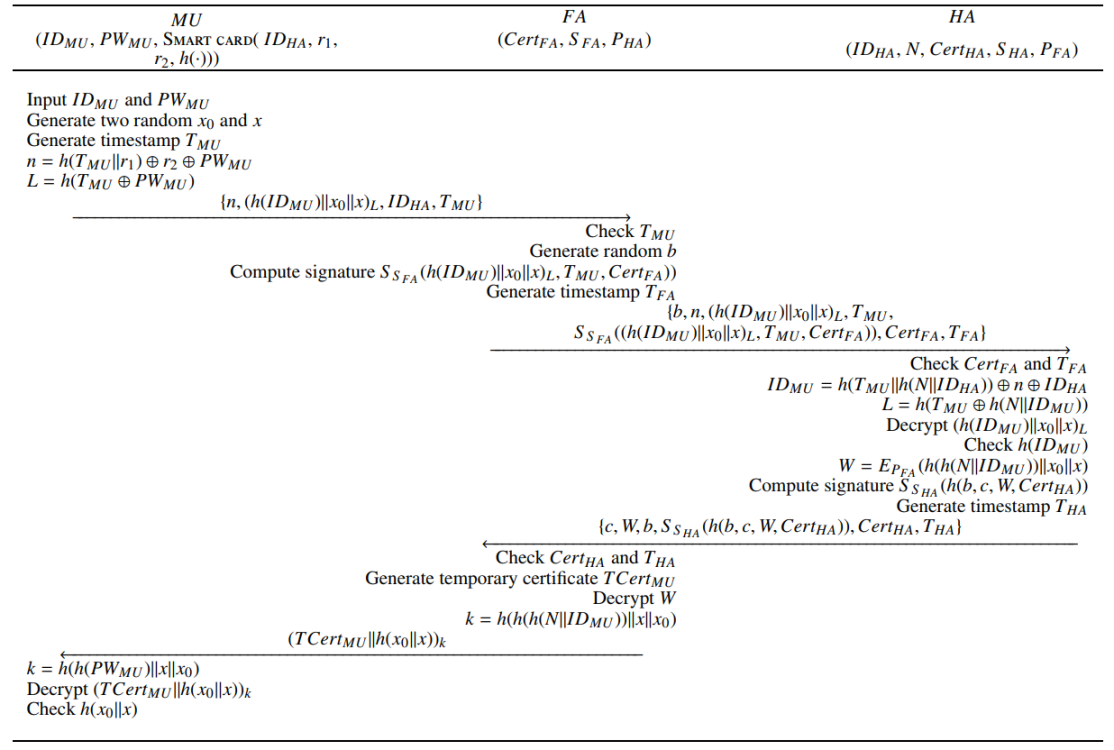
\includegraphics[width=3in]{Fig//figure.png}%尺寸要改
    \caption{First phase of Kang et al.'s scheme.}
    \end{figure}
\item \emph{FA}$\rightarrow$ \emph{HA}: 
$\{b,n,(h({ID}_{MU})||x_0||x)_L,T_{MU},{S}_{S_{FA}}, ((h({ID}_{MU}) \\ ||x_0||x)_L,T_{MU},{Cert}_{FA}
),{Cert}_{FA},T_{FA}\}$\\
    FA checks the validity of $T_{MU}$. If it is valid, then FA chooses secret random number b. FA
    then sends b, the MU’s login message containing ${n,(h({ID}_{MU})||x_0||x)_L,{ID}_{HA}, T_{MU}}$, a certificate $Cert_{FA}$, timestamp $T_{FA}$, and the corresponding signature on the
    login message by using FA’s private key $S_{FA}$to HA.
%3
\item \emph{HA}$\rightarrow$ \emph{FA}: $\{c,W,b,S_{S_{HA} (h(b,c,W,{Cert}_{HA})),{Cert}_{HA},T_{HA}}\}$\\
   \emph{ HA} checks the validity of certificate $Cert_{FA}$ and timestamp $T_{FA}$. If they are valid, then \emph{HA }computes \emph{MU}’s real identity ${ID}_{MU}$ as follows.
   \begin{eqnarray}
    ID_{MU}=h(T_{MU} ||h(N||ID_{HA}))\oplus n \oplus ID_{HA}
   \end{eqnarray}
    \emph{HA} computes \emph{$L = h(T_{MU}\oplus h(N||{ID}_{MU}))$} with his/hersecret \emph{N} and decrypts $(h({ID}_{MU})||x_0||x)_L$. Then, \emph{HA } verifies if \emph{MU} is a legal user by checking \emph{$h({ID}_{MU}) =h({ID}_{MU})'$} , where $h({ID}_{MU})$ is computed with \emph{${ID}_{MU}$} on the login message and $h({ID}_{MU})'$ of the decrypting result $\{h({ID}_{MU})'||{x_0}'||x'\}$. If so, then \emph{HA} computes $W =E_{P_{FA}}(h(h(N||{ID}_{MU}))||x_0||x)$ and generates its signature using his/her private key $S_{HA}$. Then, \emph{HA} sends random number $c, W$, the certificate of \emph{HA}, ${Cert}_{HA}$, current timestamp $T_{HA}$, and signature $S_{S_{HA}} (h(b,c,W,{Cert}_{HA}))$ to \emph{FA}.

\item \emph{FA}$\rightarrow$ \emph{MU}: $(T{Cert}_{MU}||h(x_0||x))_k$\\
    \emph{FA} checks whether or not the certificate ${Cert}_{HA}$ and timestamp $T_{HA}$ are valid. If they are valid, then \emph{FA} issues the emporary certificate $T{Cert}_{MU}$, which includes a timestamp and other information to \emph{MU}. To obtain $h(h(N||ID_{MU})||x_0||x)$, \emph{FA} decrypts \emph{W} with the secret key corresponding to $P_{FA}$. To establish session key $k_i$ for the \emph{i}-th session, \emph{FA} first saves $(T{Cert}_{MU}, h({PW}_{MU}),x_0)$. \emph{FA} encrypts $(T{Cert}_{MU}||h(x_0||x))$ with session key k and gives $(T{Cert}_{MU}||h(x_0||x))_k$ to \emph{MU}. Here, the session key is computed as follows.
    \begin{eqnarray}%覆盖范围不能空行
    \begin{split}
     k=&h(h(h(N||ID_{MU})||x||x_0))%%调整了一天才找到!!!
    \\=&h(h(PW_{MU}||x||x_0))
    \end{split}
    \end{eqnarray}
\item \emph{MU} computes \emph{k} and obtains $T{Cert}_{MU}$. \emph{MU} also authenticates \emph{FA} by computing $h(x_0||x)$ with the decrypted $h(x_0||x)$. Therefore, \emph{MU} can be sure that it is communicating with a legal \emph{FA}.
\end{enumerate}
\subsection{Second Phase}%2.3
\noindent When \emph{MU} visits \emph{FA} at the \emph{i}-th session, \emph{MU} sends the following login message to \emph{FA}.
%item里面不能展开数学环境,description没有缩进,坑死了,改了三个小时,心态爆炸,行内公式的设定也很狗很狗!!怎么都画不对!!
\begin{enumerate}
  \item \emph{MU}$\rightarrow$ \emph{FA}: \emph{$TCert_{MU}$},$(x_i||\emph{$TCert_{MU}$}||Other Information)_{k_i}$\\
  The new \emph{i}-th session key \emph{$k_i$} can be derived from the unexpired previous secret value\emph{$x_{i-1}$} and the fixed secret value \emph{x} as%不需要center命令
  \begin{eqnarray}
  k=h(h(h(N||ID_{MU})||x||x_{i-1}))
  \end{eqnarray}
  where \emph{i}=1,...,\emph{n}.
  \item Upon receiving a login message from \emph{MU}, \emph{FA} decrypts
  $(x_i||\emph{$TCert_{MU}$}||Other Information)_{k_i}$ with $k_i$ and newly saves ($TCert_{MU}$,\emph{h($PW_{MU}$),$x_i$}) for the next communication.
\end{enumerate}
\section{Anonymity Problem of KANG et al.s Scheme}
\noindent Kang et al. [7] improved Wu et al.’s scheme [3] and Wei et al.’s scheme [6] to provide anonymity. Based on the general interest of mobile users, user anonymity should be kept from any eavesdroppers including the foreign agents [5]. However, Kang et al.’s scheme still cannot provide anonymity. The main reason is that \emph{HA} always computes r1for each \emph{MU} with the same secret key \emph{N}. The detailed anonymity broken attack scenario is as follows.
\begin{enumerate}
\item Any legal user \emph{MU} can directly obtain $h(N||{ID}_{HA})$ from $r_1$ in his/her smart card because $r_1=h(N||{ID}_{HA})$ from the Eq.(2)
\item The legal user \emph{MU} can collect the messages ${n',(h({ID'}_{MU}||{x'}_0||x'))_{L'}},{ID}_{HA},T'_{MU}$ sent from any other legal mobile user \emph{MU'} to \emph{FA} at step (1) in the first phase(see Fig.1).From the Eqs.(1)~(4),we can see that \emph{n'} is equal to $h({T'}_{MU} ||r_1)\oplus {ID}_{HA}\oplus {ID'}_{MU}$ as follows.
\begin{eqnarray}
\begin{split}
n'=&h(T'_{MU}||r_1)\oplus {r_2}'\oplus PW'_{MU}\\
=&h(T'_{MU}||r_1)\oplus h(N||ID'_{MU})\oplus ID_{HA}\\
&\oplus ID'_{MU} \oplus PW'_{MU}\\
=&h(T'_{MU}||r_1)\oplus h(N||ID'_{MU})\oplus ID_{HA}\\
&\oplus ID'_{MU} \oplus h(N||ID'_{MU})\\
=&h(T'_{MU}||r_1)\oplus ID_{HA}\oplus ID_{MU}\oplus\\
\end{split}
\end{eqnarray}
\item With obtained $r_1=h(N||{ID}_{HA})$ and collected messages${n',{ID}_{HA},T'_{MU}}$,\emph{MU} can get the real identity ${ID'}_{MU}$ of the other mobile user \emph{MU's} as \emph{HA} does at step (3) in the first phase as follows.
\begin{eqnarray}%公式10,没有用居中命令,自然就居中了
\begin{split}
ID'_{MU}=&n'\oplus ID_{HA} \oplus h(T'_{MU}||r_1)\\
=&h(T'_{MU}||r_1)\oplus ID_{HA}\oplus ID'_{MU}\\
&\oplus ID_{HA} \oplus h(T'_{MU}||r_1)\\
=&ID'_{MU}
\end{split}
\end{eqnarray}
As a result, legal mobile user \emph{MU’s} anonymity cannot be preserved in Kang et al.’s scheme.
\end{enumerate}
\section{Conclusions}
This letter demonstrated that recently published wireless authentication scheme by Kang et al. still cannot provide anonymity. Therefore, Kang et al.’s scheme did not solved
the problem of user anonymity that was pointed out Zeng
et al. [4] and Lee et al. [5].
\section*{Acknowledgements}
This research was supported by Basic Science Research Pro-
gram through the National Research Foundation of Korea
(NRF) funded by the Ministry of Education, Science and
Technology (No. 2010-0010106) and partially supported by
the MKE (The Ministry of Knowledge Economy), Korea,
under the ITRC (Information Technology Research Center)
support program (NIPA-2012-H0301-12-2004) supervised
by the NIPA (National IT Industry Promotion Agency).
\begin{thebibliography}{00}
\bibitem{Li10}J. Zhu and J. Ma, “A new authentication scheme with anonymity for wireless environment,” IEEE Trans. Consum. Electron., vol.50, no.1, pp.230–234, 2004.
\bibitem{Li10}C.C. Lee, M.S. Hwang, and I.E. Liao, “Security enhancement on a new authentication scheme with anonymity for wireless environments,” IEEE Trans. Ind. Electron., vol.53, no.5, pp.1683–1687, 2006.
\bibitem{Li10}C.C. Wu, W.B. Lee, and W.J. Tsaur, “A secure authentication scheme with anonymity for wireless communications,” IEEE Commun. Lett., vol.12, no.10, pp.722–723, 2008.
\bibitem{Li10}P. Zeng, Z. Cao, K.R. Choo, and S. Wang, “On the anonymity of some authentication schemes for wireless communications,” IEEE Commun. Lett., vol.13, no.3, pp.170–171, 2009.
\bibitem{Li10}J. Lee, J.H. Chang, and D.H. Lee, “Security flaw of authentication scheme with anonymity for wireless communications,” IEEE Commun. Lett., vol.13, no.5, pp.292–293, 2009.
\bibitem{Li10}Y. Wei, H. Qiu, and Y. Hu, “Security analysis of authentication scheme with anonymity for wireless environments,” ICCT (International Conference on Communication Technology), 2006.
\bibitem{Li10} M. Kang, H. Rhee, and J. Choi, “Improved user authentication scheme with user anonymity forwireless communications,” IEICE Trans. Fundamentals, vol.E94-A, no.2, pp.860–864, Feb. 2011.
\end{thebibliography}
%the bibliography environment
%引用一篇文章\cite{article1}\\%所有需要交叉引用的地方都需要编译两次,第一次是问号
\end{document}